\documentclass[conference]{IEEEtran}
\usepackage[T1]{fontenc}
\usepackage{amsmath,amssymb}
\usepackage{graphicx}
\usepackage{booktabs}
\usepackage{xcolor}
\usepackage{url}
\usepackage[hidelinks]{hyperref}


\begin{document}

\title{Where the Time Goes: A GPU Bottleneck Study\\ of the Duan et al.\ Shortest Path Algorithm}

\author{
\IEEEauthorblockN{Siddhanth Methil, Siddharth Prabhu, Aryan K Shetty, Shetty Aniketh Nishikanth}
\IEEEauthorblockA{Department of Computer Science and Engineering\\
Manipal Institute of Technology, Manipal Academy of Higher Education, Manipal, India}
}

\maketitle

\begin{abstract}
Duan et al.\ (STOC 2025) gave the first deterministic algorithm for directed single-source shortest paths (SSSP) that
beats the $O(m + n\log n)$ bound of Dijkstra's algorithm on sparse graphs. In practice it is still several times slower
than Dijkstra's algorithm. We ask whether a GPU can close this gap. The algorithm's FindPivots step runs Bellman-Ford
rounds, which is the part that maps best to a GPU. We implement it on the GPU inside the reference implementation and
verify every GPU call against a CPU reference. On five road, grid and R-MAT graphs, the GPU version is between
0.25$\times$ and 1.03$\times$ as fast as the CPU version. A per-call cost model explains this. FindPivots takes only
12--22\% of the run, and its median call examines 181 to 12{,}723 edges, while a GPU call has a fixed cost of
69--122\,\textmu s. A time breakdown then shows a stronger limit. The algorithm's sequential data structure alone takes
2.2--3.8 times as long as a complete run of Dijkstra's algorithm. It stays above one Dijkstra run on every graph up to
$2^{22}$ vertices. Batching FindPivots calls across concurrent searches gains at most 7\%, and only when the GPU worker thread
gets a core of its own. That core is worth more as a CPU core. A GPU Near-Far SSSP is 11--24 times faster than
Dijkstra's algorithm on R-MAT graphs, which shows that the GPU itself is not the problem.
\end{abstract}

\begin{IEEEkeywords}
single-source shortest paths, GPU, CUDA, Bellman-Ford, performance analysis, Amdahl's law
\end{IEEEkeywords}

\section{Introduction}

Dijkstra's algorithm with a Fibonacci heap solves SSSP on a directed graph with non-negative weights in
$O(m + n\log n)$ time. This bound was long seen as a barrier, since Dijkstra's algorithm also sorts the vertices by
distance. Duan, Mao, Mao, Shu and Yin broke it with a deterministic $O(m\log^{2/3} n)$ algorithm~\cite{duan2025}, and
the same group has since lowered the bound again~\cite{duan2026}.

The new algorithm is not yet fast in practice. Castro et al.\ implemented it in C++ and found that Dijkstra's algorithm
stays 3 to 4 times faster on every graph they tested~\cite{castro2025}. The algorithm contains Bellman-Ford rounds,
and Bellman-Ford maps well to GPUs. This suggests a practical question: can a GPU remove enough of the constant factor
to make the algorithm competitive?

We answer this question by measurement. We keep the reference implementation of Castro et al.\ on the CPU and replace
its Bellman-Ford step with a GPU version. We then measure where the time goes, and how much any GPU offload could save.

\paragraph{Contributions.} We make five contributions.
\begin{itemize}
\item A GPU FindPivots that plugs into the reference implementation, and a batched version that serves several
concurrent searches with one set of kernel launches. Both give exactly the same result as a serial reference on every
call we checked. To our knowledge, these are the first GPU implementations of any part of the algorithm.
\item A per-call cost model with two upper bounds on the speedup that a GPU FindPivots can give.
\item A time breakdown of the whole algorithm, which shows that its sequential data structure alone costs more than
Dijkstra's algorithm.
\item A test of batching across searches, with the gain predicted from single-search data before the run.
\item A comparison with Dijkstra's algorithm on the CPU and a tuned GPU Near-Far SSSP~\cite{davidson2014}, and a
scaling study from $2^{14}$ to $2^{22}$ vertices.
\end{itemize}

\section{Background}

\paragraph{The Duan et al.\ algorithm.} The algorithm is a recursive procedure called bounded multi-source shortest
path (BMSSP). A call $\mathrm{BMSSP}(l, B, S)$ finds the shortest paths below a bound $B$ from a set $S$ of frontier
vertices. The parameters are $k = \lfloor \log^{1/3} n \rfloor$ and $t = \lfloor \log^{2/3} n\rfloor$, with
$\lceil \log n / t\rceil$ recursion levels. Each call first runs FindPivots, which does $k$ rounds of Bellman-Ford
relaxation from $S$ below $B$. If the set $W$ of reached vertices grows beyond $k|S|$, it stops early. Otherwise it
returns as pivots $P$ only the vertices of $S$ whose shortest-path trees in $W$ hold at least $k$ vertices. The call
puts $P$ into a partial-sorting data structure $D$, pulls batches of the closest vertices from $D$, and recurses on
each batch. After each recursive call it relaxes the out-edges of the vertices that call completed, and inserts or
prepends the improved vertices into $D$. Only pivots enter $D$, so $D$ holds about $|S|/k$ vertices instead of $|S|$.
This is how the algorithm avoids a full sort.

\paragraph{Why FindPivots is the GPU candidate.} Most of the algorithm is a sequence of dependent operations on $D$, and
each recursive call depends on the batch before it. FindPivots is different. Each round relaxes all out-edges of the
current frontier, and these relaxations are independent. This is the pattern that GPU SSSP methods use.

\paragraph{GPU SSSP.} Delta-stepping~\cite{meyer2003} groups vertices into buckets of width $\Delta$ and relaxes each
bucket in parallel. Near-Far~\cite{davidson2014} keeps only two buckets, near and far, and is a standard work-efficient
GPU method. Later work such as ADDS adapts the bucket width at run time~\cite{wang2021}. These methods keep the whole
computation on the GPU and process large frontiers in each step.

\section{Design}

\paragraph{Overview.} The hybrid keeps the BMSSP recursion, the data structure $D$ and the base case on the CPU. We use
the single-header C++ implementation of Castro et al.~\cite{castro2025} (its worst-case variant) with an
instrumentation layer. A hook replaces each FindPivots call. It measures the first-round edge work $w_0$, the sum of the
out-degrees of $S$. If $w_0$ reaches a threshold, the call runs on the GPU. Otherwise it runs on the CPU. The graph is
copied to the GPU once, in compressed sparse row form.

\paragraph{Synchronous rounds.} The CPU reference relaxes edges in place, so a vertex improved early in a round can be
relaxed again in the same round. A GPU cannot reproduce this order. We therefore use synchronous rounds: every
proposal in a round reads the state at the start of the round. A vertex can receive several proposals in one round,
and the winner is the lexicographic minimum of (distance, hop count, predecessor), which is the tie-breaking key of the
reference implementation. With this rule, the result of a round depends only on its input state. A serial CPU version
with the same semantics is our correctness reference and the \emph{sync\_cpu} configuration.

\paragraph{Kernels.} One round runs four kernels over the active list. Pass~1 uses one thread per out-edge, and each
improving proposal does an \texttt{atomicMin} on a candidate distance. In pass~2, the proposals that hold the winning
distance do one 64-bit \texttt{atomicMin} on the packed value $(\mathit{hops} \ll 32) \mid \mathit{pred}$. Two commit
kernels then write the winners. A winner whose key is below $B$ joins the next active list and inherits the tree root
of its predecessor. We split the commit into two kernels so that no thread reads the root array while another thread
writes it. Each round needs one copy to the GPU (edge offsets and active list together) and one small copy back.

\paragraph{State ownership.} The CPU changes distances between FindPivots calls. Uploading all $n$ vertices before each
call would cost more than the call itself. We therefore record every vertex the CPU changes, through the single update
function of the reference implementation, and upload only those vertices. After the call, only the vertices the GPU
changed are copied back. On R-MAT20 this reduces the uploaded vertices from 284 million to 2.2 million per run.

\paragraph{Batching across searches.} Several independent searches can share the GPU. Each search runs in its own CPU
thread, and one worker thread owns the GPU. When the GPU is free, the worker takes every waiting FindPivots call and
runs them as one batch. We treat the searches as disjoint copies of the graph: vertex $v$ of search $i$ is
$i\cdot n + v$, and the graph is stored once. One set of kernel launches then serves the whole batch, and each call
keeps its own bound, early exit, $W$ and $P$. A waiting thread sleeps instead of spinning, so that other searches can
use its core.

\paragraph{Near-Far baseline.} We implement Near-Far fully on the GPU. A CUB exclusive scan of the frontier degrees
assigns one thread to each frontier edge. Each thread does an \texttt{atomicMin} on the distance and appends an
improved vertex to the next near frontier or to the far pile. When the near frontier is empty, the split moves up by
$\Delta$. We sweep $\Delta$ from $1/16$ to $32$ times the average edge weight on R-MAT, where the time is flat at the top
of this range, and from $1/16$ to $4096$ times on NY and Grid500. We report the best value per graph.

\section{Verification}

A fast but wrong kernel would make every timing meaningless, so we verify before we measure.

\paragraph{Per-call equivalence.} In check mode, the driver copies the solver state before each GPU call, runs the
serial synchronous version, restores the state and runs the GPU version. It then compares $P$, the order of $W$, and
the full distance, predecessor and hop arrays. The batched version does the same for every call in every batch. Final
distances are also compared with an independent binary-heap Dijkstra.

\paragraph{Coverage.} On the GPU, the single-search version passed 149 of 149 check runs with 47{,}271 GPU calls,
on the five graphs and 38 small random and grid graphs. The batched version passed 91 of 91 runs with 94{,}984 batched calls. Near-Far
matched Dijkstra in 139 of 139 runs, each with 11 values of $\Delta$.

\paragraph{Mutation tests.} We plant bugs to check that the method can fail. A last-writer-wins predecessor update is
caught on the fourth call. Merging the two commit kernels, which creates a race on the root array, is caught in 2 of 228
emulated fuzz runs. In the batched version, a root taken from the wrong search, the bound of the wrong search, a
write-back to the wrong search, and an early exit that does not stop the search are each caught.

\section{Experimental Setup}

\paragraph{Hardware and software.} We use a laptop with an AMD Ryzen 5 4600H (6 cores, 12 threads) and an NVIDIA
GeForce GTX 1660 Ti (Turing, 6\,GB). Host code is compiled with GCC 15.3 and device code with CUDA 13.0, both with
\texttt{-O3}.

\paragraph{Graphs.} Table~\ref{tab:graphs} lists the graphs. NY is the DIMACS road network of New York with distance
weights. Grid500 is a $500\times 500$ four-neighbour grid. The R-MAT graphs use parameters (0.57, 0.19, 0.19, 0.05)
and eight edges per vertex. The synthetic graphs have integer weights from 1 to 100. All five graphs have $k = 2$, so a
FindPivots call runs at most two rounds.

\begin{table}[t]
\centering
\footnotesize\setlength{\tabcolsep}{3pt}
\caption{Test graphs and BMSSP parameters.}
\label{tab:graphs}
\begin{tabular}{lrrrrrr}
\toprule
Graph & $n$ & $m$ & $k$ & $t$ & Levels & Calls per run \\
\midrule
NY & 264{,}346 & 733{,}846 & 2 & 6 & 4 & 4{,}036 \\
Grid500 & 250{,}000 & 998{,}000 & 2 & 6 & 3 & 3{,}784 \\
R-MAT16 & 65{,}536 & 524{,}288 & 2 & 6 & 3 & 149 \\
R-MAT18 & 262{,}144 & 2{,}097{,}152 & 2 & 6 & 3 & 183 \\
R-MAT20 & 1{,}048{,}576 & 8{,}388{,}608 & 2 & 7 & 3 & 305 \\
\bottomrule
\end{tabular}
\end{table}

\paragraph{Method.} Each graph has five random sources that reach at least 10\% of the vertices. Each (graph, source)
pair runs five repetitions of every configuration, each in a fresh process, in a shuffled order. We report the median
execute time, which excludes graph loading and GPU setup. All configurations of a (graph, source) pair must produce the
same distances, and we hash the output to check this. The configurations are \emph{builtin} (the unmodified reference),
\emph{cpu\_hooked} (hook and change tracking installed, every call on the CPU), \emph{gpu\_all} (every call on the GPU)
and \emph{gpu\_tX} (calls with $w_0 \ge X$ on the GPU). The hook and the change tracking alone shift the run time by
$-4.5\%$ to $+4.7\%$ against \emph{builtin}. We therefore measure the effect of the GPU against \emph{cpu\_hooked},
which has the same process setup.

\section{Results}

\subsection{End-to-end time}

Table~\ref{tab:e2e} shows that no GPU configuration is clearly faster than the CPU. Running every call on the GPU makes
BMSSP about four times slower on NY and Grid500. With a threshold of 4{,}096 edges, almost no calls reach the GPU on
these graphs, so the time equals the CPU time. On R-MAT20, the GPU takes 271 of 305 calls and the run is 2.6\% faster.
This is the largest gain we measured.

\begin{table}[t]
\centering
\footnotesize\setlength{\tabcolsep}{3pt}
\caption{Median execute time (ms) of the CPU runs, and speedup of the GPU configurations over \emph{cpu\_hooked}
(paired per source and repetition). \emph{hooked} = \emph{cpu\_hooked}; tX = \emph{gpu\_tX}.}
\label{tab:e2e}
\begin{tabular}{lrrrrrr}
\toprule
Graph & Dijkstra & builtin & hooked & gpu\_all & t4096 & t16384 \\
\midrule
NY & 25.0 & 137.7 & 131.1 & 0.28$\times$ & 1.00$\times$ & 1.00$\times$ \\
Grid500 & 33.2 & 121.4 & 117.5 & 0.25$\times$ & 1.00$\times$ & 1.00$\times$ \\
R-MAT16 & 11.2 & 58.8 & 61.7 & 0.84$\times$ & 0.95$\times$ & 1.00$\times$ \\
R-MAT18 & 60.6 & 297.1 & 309.5 & 0.98$\times$ & 0.99$\times$ & 1.00$\times$ \\
R-MAT20 & 314.9 & 1403.0 & 1448.1 & 1.02$\times$ & 1.03$\times$ & 1.02$\times$ \\
\bottomrule
\end{tabular}
\end{table}

\subsection{How much can a GPU FindPivots save?}

The GPU FindPivots and the synchronous CPU version have the same semantics, so their call sequences are identical. We
use this to pair the calls one to one and compute two bounds from the logs of the \emph{sync\_cpu} runs. Let $T$ be the
run time and $F$ the total FindPivots time. If FindPivots cost nothing, the run would take $T - F$. If each call used the
faster of its measured CPU and GPU times, the run would take $T - F + \sum_i \min(c_i, g_i)$.

Table~\ref{tab:bounds} and Fig.~\ref{fig:model} show both bounds. FindPivots takes only 12--22\% of the run, so even a
free FindPivots gives at most 1.29$\times$. With the measured GPU costs, the best per-call choice gives at most
1.056$\times$, on R-MAT20. On NY the GPU is faster in none of the 4{,}036 calls of a run, and on Grid500 in one.

\begin{table}[t]
\centering
\footnotesize\setlength{\tabcolsep}{3pt}
\caption{Upper bounds on the speedup over \emph{sync\_cpu} (median over five sources).}
\label{tab:bounds}
\begin{tabular}{lrrrr}
\toprule
Graph & FindPivots share & Free FindPivots & Best per-call & GPU faster \\
\midrule
NY & 17.9\% & 1.22$\times$ & 1.000$\times$ & 0 of 4{,}036 \\
Grid500 & 22.3\% & 1.29$\times$ & 1.000$\times$ & 1 of 3{,}784 \\
R-MAT16 & 11.7\% & 1.13$\times$ & 1.009$\times$ & 9 of 149 \\
R-MAT18 & 13.1\% & 1.15$\times$ & 1.037$\times$ & 61 of 183 \\
R-MAT20 & 13.3\% & 1.15$\times$ & 1.056$\times$ & 220 of 305 \\
\bottomrule
\end{tabular}
\end{table}

\begin{figure}[t]
\centering
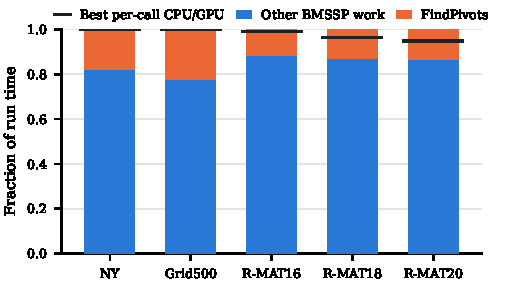
\includegraphics[width=\columnwidth]{fig/model.pdf}
\caption{Share of FindPivots in the \emph{sync\_cpu} run time, and the run time with the best per-call CPU/GPU choice
(black line). Median over five sources.}
\label{fig:model}
\end{figure}

\subsection{Why the GPU calls are slow}

Fig.~\ref{fig:percall} shows the median time per call against $w_0$. The CPU time grows with the work, from under
1\,\textmu s. The GPU time has a floor that does not depend on the work. We fit each phase of a GPU call separately
(upload, rounds and download). The fixed part of a two-round call is 69--122\,\textmu s, after we merged the per-round
copies. An earlier version had 114--176\,\textmu s. Above the floor, the GPU costs 2.8--5.3\,ns per edge on R-MAT,
against 16--21\,ns per edge on the CPU. A call therefore pays off on the GPU above about 4{,}700--6{,}400 edges.

The calls are much smaller than this. The median call examines 181 edges on NY, 263 on Grid500, 1{,}832 on R-MAT16,
5{,}955 on R-MAT18 and 12{,}723 on R-MAT20. The cause is structural: FindPivots runs at most $k = 2$ rounds and stops early
once $|W| > k|S|$. On NY and Grid500, the recursion makes about 4{,}000 such calls in sequence, and each depends on the
previous one through $D$. Their per-edge GPU cost cannot even be fitted, because almost all of a call's time is the
floor.

\paragraph{Model check.} We fit the phase costs on four graphs and predict the total GPU FindPivots time of the fifth
from its logged call sizes. The error is within 16\% for four graphs. On R-MAT20 the model predicts 32\% too little,
because the per-vertex cost of upload and download grows on the largest graph.

\begin{figure}[t]
\centering
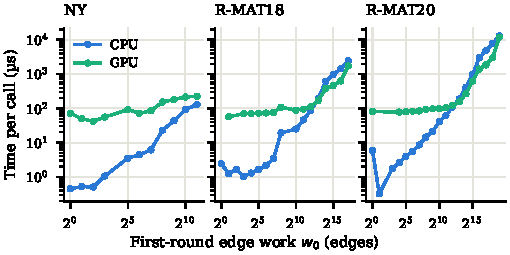
\includegraphics[width=\columnwidth]{fig/per_call.pdf}
\caption{Median time per FindPivots call against its first-round edge work, synchronous CPU and GPU, over five sources. The
first GPU call, which uploads the full state, is left out.}
\label{fig:percall}
\end{figure}

\subsection{Where the rest of the time goes}

FindPivots is a small part of the run, so we measure the rest. The reference implementation already times the
base case, the pulls and batch prepends on $D$, and the relax loop after each recursive call. The relax loop mixes edge
scanning with inserts and erases on $D$. Timers around each operation would distort the run. On NY they added about
50\%. We therefore record every operation on $D$ in a second run, replay the recording on fresh $D$ objects, and time
each kind of operation. Each replayed pull is checked against the recorded one with a hash of the pulled vertices,
which catches three planted replay bugs. Where the reference implementation also times an operation (pulls and
prepends), the replayed time agrees with it: the median ratio per graph is 0.88 to 1.06.

Table~\ref{tab:breakdown} and Fig.~\ref{fig:breakdown} split each run into $D$ operations, edge work (FindPivots, base
case, and edge scanning in the relax loop) and the rest. The operations on $D$ alone take 2.2--3.8 times as long as a
complete run of Dijkstra's algorithm on the same graph and source. All edge work together is 25--43\% of the run. If a
GPU made all of it free, BMSSP would be at most 1.34--1.75$\times$ faster, and still 2.4--4.3 times slower than
Dijkstra's algorithm.

\begin{table}[t]
\centering
\footnotesize\setlength{\tabcolsep}{3pt}
\caption{BMSSP time breakdown against Dijkstra (ms, median over five sources, ratios paired per source).}
\label{tab:breakdown}
\begin{tabular}{lrrrrr}
\toprule
Graph & Dijkstra & BMSSP & $D$ ops & $D$ / Dijkstra & Edge work free \\
\midrule
NY & 25.6 & 139.8 & 70.1 & 2.69$\times$ & 1.75$\times$ \\
Grid500 & 34.7 & 123.3 & 77.2 & 2.21$\times$ & 1.39$\times$ \\
R-MAT16 & 10.5 & 60.0 & 40.4 & 3.84$\times$ & 1.34$\times$ \\
R-MAT18 & 59.8 & 308.0 & 215.4 & 3.58$\times$ & 1.34$\times$ \\
R-MAT20 & 343.2 & 1570.4 & 1063.7 & 3.17$\times$ & 1.36$\times$ \\
\bottomrule
\end{tabular}
\end{table}

\begin{figure}[t]
\centering
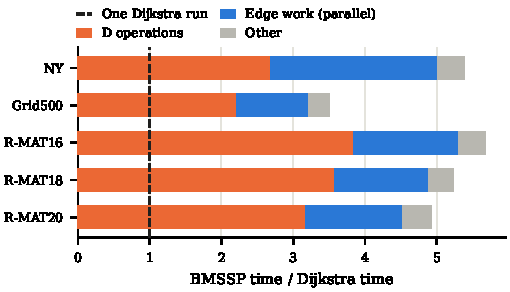
\includegraphics[width=\columnwidth]{fig/breakdown.pdf}
\caption{BMSSP run time in units of one Dijkstra run, split into operations on $D$, edge work that a GPU could run in
parallel, and other work. Median over five sources.}
\label{fig:breakdown}
\end{figure}

\subsection{Batching FindPivots across searches}

Batching shares the fixed cost of a GPU call between searches, but each search still waits for its own call. With one
core per search, a waiting search leaves its core idle, so batching cannot hide the wait. A gain needs more searches
than cores, so that other searches use the core during the wait. We test both cases: 5 searches with a core each, and
8 searches on 2 physical cores.

Before running them, we predicted both cases with an event simulation built from the single-search data. Each search
replays the logged calls and CPU work of a real run, the searches share the cores, and a batch costs the fixed part of a
call once plus each call's own variable part. Fig.~\ref{fig:batching} compares the prediction with the measurement. The
prediction was a gain of at most 9\% (R-MAT20, 8 searches on 2 cores). We measured no gain in any case: the speedup over
CPU FindPivots in the same setting was 0.11--0.95$\times$ with 5 searches and 0.18--0.98$\times$ with 8.

The prediction was too optimistic for two reasons we can show. First, the batched code path costs more per call than the
single-search one, even with nothing to batch: with one search, it adds 69--537\,\textmu s per call. Second, with 8
searches on 2 cores, the GPU worker thread competes with the searches for the same cores, which the model leaves out.

\paragraph{Removing the two causes.} We then removed each cause in turn (Table~\ref{tab:diag}). Letting the worker
spin-wait on the GPU, instead of sleeping until the GPU wakes it, removes most of the extra cost: one search on NY drops
from 943 to 511\,ms, close to the single-search hybrid. Giving the worker a core of its own removes the contention.
With both changes, 8 searches on 2 cores reach 0.47--1.07$\times$ the CPU version, within 2--10\% of the prediction
(0.51--1.09$\times$). The model is therefore right once its two assumptions hold. This setting, however, uses a third
core for the worker. Given that core as a third CPU core instead, the CPU version is faster on every graph. On R-MAT20 it
takes 5{,}560\,ms, against 6{,}905\,ms for the best GPU setting.

\begin{table}[t]
\centering
\footnotesize\setlength{\tabcolsep}{3pt}
\caption{Eight searches, wall time (ms, median over three repetitions). GPU: batched FindPivots; the worker sleeps or
spins while waiting, and in the last GPU column it has a third core of its own.}
\label{tab:diag}
\begin{tabular}{lrrrrr}
\toprule
 & CPU & GPU, sleep & GPU, spin & GPU, spin & CPU \\
Graph & 2 cores & 2 cores & 2 cores & 2+1 cores & 3 cores \\
\midrule
NY & 707 & 3{,}659 & 1{,}883 & 1{,}352 & 539 \\
Grid500 & 597 & 3{,}272 & 1{,}698 & 1{,}255 & 456 \\
R-MAT16 & 320 & 452 & 388 & 353 & 253 \\
R-MAT18 & 1{,}585 & 1{,}814 & 1{,}653 & 1{,}569 & 1{,}235 \\
R-MAT20 & 7{,}350 & 7{,}378 & 7{,}189 & 6{,}905 & 5{,}560 \\
\bottomrule
\end{tabular}
\end{table}

\begin{figure}[t]
\centering
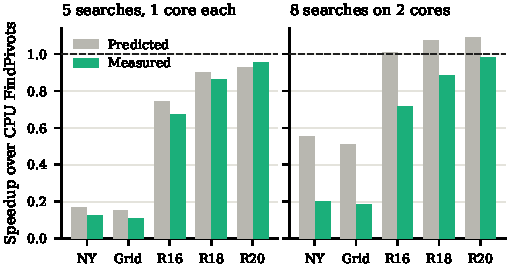
\includegraphics[width=\columnwidth]{fig/batching.pdf}
\caption{Speedup of batched GPU FindPivots over CPU FindPivots in the same setting, predicted from single-search data
before the run, and measured. Median over three repetitions. R16--R20: R-MAT16--20; Grid: Grid500.}
\label{fig:batching}
\end{figure}

\subsection{Comparison with a GPU SSSP}

Table~\ref{tab:nearfar} compares Dijkstra's algorithm with Near-Far at its best $\Delta$. On R-MAT graphs, Near-Far is
11--24 times faster than Dijkstra's algorithm. On R-MAT20 it takes 13.1\,ms, against 1{,}403\,ms for BMSSP. On NY and
Grid500 it is slower than Dijkstra's algorithm, as expected for graphs with a large diameter and small frontiers. The GPU
is therefore not the obstacle. The obstacle is the shape of the work that BMSSP gives it.

\begin{table}[t]
\centering
\footnotesize\setlength{\tabcolsep}{3pt}
\caption{Dijkstra (CPU) against Near-Far (GPU) at its best $\Delta$, given as a multiple of the average edge weight.
Median execute time in ms.}
\label{tab:nearfar}
\begin{tabular}{lrrrr}
\toprule
Graph & Dijkstra & BMSSP & Near-Far ($\Delta$) & Dijkstra / Near-Far \\
\midrule
NY & 25.0 & 137.7 & 48.0 (256$\times$) & 0.52$\times$ \\
Grid500 & 33.2 & 121.4 & 38.6 (64$\times$) & 0.86$\times$ \\
R-MAT16 & 11.2 & 58.8 & 1.0 (8$\times$) & 11.2$\times$ \\
R-MAT18 & 60.6 & 297.1 & 2.8 (32$\times$) & 21.7$\times$ \\
R-MAT20 & 314.9 & 1403.0 & 13.1 (0.5$\times$) & 24.0$\times$ \\
\bottomrule
\end{tabular}
\end{table}

\subsection{Scaling}

The theory predicts that BMSSP closes in on Dijkstra's algorithm as graphs grow: binary-heap Dijkstra takes
$O(m\log n)$ time and BMSSP $O(m\log^{2/3} n)$, so their time ratio should fall like $\log^{-1/3} n$. We test this on
generated R-MAT graphs with $2^{14}$ to $2^{22}$ vertices and grids from $128^2$ to $2048^2$ vertices, with the same
parameters and weights as the test graphs and three sources each (Fig.~\ref{fig:scaling}).

The ratio does not fall in a consistent way. On R-MAT it drops from 6.4 at $2^{14}$ to 5.0 at $2^{20}$, then rises to
5.5 at $2^{22}$. On grids it stays between 4.0 and 4.4 up to $2^{20}$ and rises to 5.2 at $2^{22}$. Both algorithms get
slower per edge as the graphs outgrow the caches, and BMSSP more so: on R-MAT, Dijkstra goes from 16 to 43\,ns per edge
and BMSSP from 104 to 235\,ns. On R-MAT the operations on $D$ fall from 5.0 to 3.5 Dijkstra runs, but they stay above one
Dijkstra run at every size. A fit of the ratio to $a(\log_2 n)^b$ gives $b = -0.51$ on R-MAT ($R^2 = 0.67$) and
$b = +0.26$ on grids ($R^2 = 0.14$). Taken at face value, the R-MAT fit reaches a ratio of 1 only at
$\log_2 n \approx 522$, and the grid fit never does. Both agree with the estimate of Castro et al.\ that the crossover
lies far beyond any real graph~\cite{castro2025}.

\begin{figure}[t]
\centering
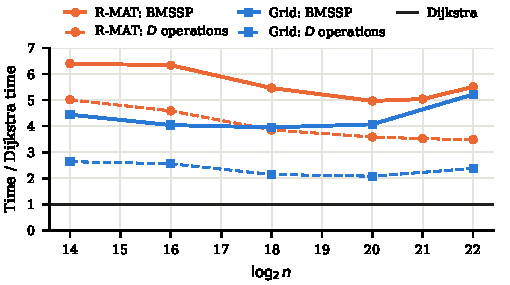
\includegraphics[width=\columnwidth]{fig/scaling.pdf}
\caption{BMSSP time and the time of its operations on $D$, in units of one Dijkstra run, on generated R-MAT graphs and
grids. Median over three sources.}
\label{fig:scaling}
\end{figure}

\section{Discussion}

\paragraph{The obstacle is granularity.} A GPU needs large, independent units of work to cover its fixed costs. Near-Far
gets them by relaxing whole buckets of vertices in each step. The Duan et al.\ algorithm reaches its bound by doing the
opposite: it keeps frontiers small so that $D$ stays small. The idea that gives the better bound is the same idea that
removes the parallel work. A faster kernel cannot change this, because the floor comes from launches, synchronization
and transfers, not from the relaxations.

\paragraph{The data structure is the real cost.} Even with all parallel work removed, the operations on $D$ cost more
than Dijkstra's algorithm. A practical version of the algorithm therefore needs a cheaper $D$ first. In the reference
implementation, $D$ is a linked list of blocks with a balanced tree of block bounds and hash maps. Each insert or
erase costs several pointer-chasing steps, against one cache-friendly heap operation in Dijkstra's algorithm.

\paragraph{Limitations.} We measure one laptop GPU and CPU, one implementation of the algorithm (the worst-case variant
of Castro et al.), and graphs with $k = 2$. A larger $k$ would give longer FindPivots calls, but $k$ grows as
$\log^{1/3} n$ and reaches 3 only at $n = 2^{27}$. Our batching runs one search per CPU thread. Running several searches
per thread could hide the wait differently.

\section{Conclusion}

We built and verified a GPU FindPivots for the Duan et al.\ SSSP algorithm, measured it inside the reference
implementation, and tested batching across searches. None of them make the algorithm competitive. FindPivots is a
small part of the run, its calls are much smaller than the size at which a GPU call pays off, and the sequential data
structure alone costs more than Dijkstra's algorithm, at every size we tested. The method we used, per-call logs, bounds, an operation replay and a
prediction made before the run, applies to other recursive algorithms that call a parallel subroutine many times.

\section*{Acknowledgment}
We thank Dr.\ G.\ Arul Elango for guidance, and L.\ Castro, T.\ Clementino and R.\ de Freitas for their public
implementation.

\begin{thebibliography}{9}
\bibitem{duan2025} R.~Duan, J.~Mao, X.~Mao, X.~Shu, and L.~Yin, ``Breaking the sorting barrier for directed
single-source shortest paths,'' in \emph{Proc.\ 57th Annu.\ ACM Symp.\ Theory of Computing (STOC)}, 2025.
arXiv:2504.17033.
\bibitem{duan2026} R.~Duan, X.~Mao, X.~Shu, and L.~Yin, ``A faster directed single-source shortest path algorithm,''
arXiv:2602.07868, 2026.
\bibitem{castro2025} L.~Castro, T.~Clementino, and R.~de~Freitas, ``Implementation and brief experimental analysis of
the Duan et al.\ (2025) algorithm for single-source shortest paths,'' arXiv:2511.03007, 2025.
\bibitem{meyer2003} U.~Meyer and P.~Sanders, ``$\Delta$-stepping: A parallelizable shortest path algorithm,''
\emph{J.\ Algorithms}, vol.~49, no.~1, pp.~114--152, 2003.
\bibitem{davidson2014} A.~Davidson, S.~Baxter, M.~Garland, and J.~D.~Owens, ``Work-efficient parallel GPU methods for
single-source shortest paths,'' in \emph{Proc.\ IEEE IPDPS}, 2014.
\bibitem{wang2021} K.~Wang, D.~Fussell, and C.~Lin, ``A fast work-efficient SSSP algorithm for GPUs,'' in
\emph{Proc.\ ACM PPoPP}, 2021.
\end{thebibliography}

\end{document}
